\documentclass[11pt,a4paper,titlepage]{article}
\usepackage[utf8x]{inputenc}
\usepackage[T1]{fontenc}
%\usepackage{gentium}
\usepackage{mathptmx} % Use Times Font
\usepackage{amsmath}


\usepackage[pdftex]{graphicx} % Required for including pictures
\usepackage[english]{babel} % Swedish translations
\usepackage[pdftex,linkcolor=black,pdfborder={0 0 0}]{hyperref} % Format links for pdf
\usepackage{calc} % To reset the counter in the document after title page
\usepackage{enumitem} % Includes lists

\frenchspacing % No double spacing between sentences
\linespread{1.2} % Set linespace
\usepackage[a4paper, lmargin=0.1666\paperwidth, rmargin=0.1666\paperwidth, tmargin=0.1111\paperheight, bmargin=0.1111\paperheight]{geometry} %margins
%\usepackage{parskip}

\usepackage[all]{nowidow} % Tries to remove widows
\usepackage[protrusion=true,expansion=true]{microtype} % Improves typography, load after fontpackage is selected

%-----------------------
% Set pdf information and add title, fill in the fields
%-----------------------
\hypersetup{ 	
pdfsubject = {},
pdftitle = {},
pdfauthor = {}
}

%-----------------------
% Begin document
%-----------------------

\begin{document} %All text i dokumentet hamnar mellan dessa taggar, allt ovanför är formatering av dokumentet
\bibliographystyle{ieeetr}

\begin{titlepage}
  \centering
  \vspace*{2cm}
  {\Huge \textbf{\underline{CS-E4840}}}\\[0.5cm]
  {\Huge \textbf{\underline{\parbox{0.8\linewidth}{\centering Information Visualization D}}}}\\[1.0cm]
  {\Large \textbf{Assignment 4: Advanced Topics}} \\
  [1.0cm]
  {\Large Aleksi Kääriäinen (728971)}\\[1.0cm]
  {\Large \today}
\end{titlepage}

\section*{Introduction}

In this assignment, I have completed two visualization tasks using data relating to the SDG selected in assignment 1. Restating just for clarity, I picked SDG number 1, No poverty, for the topic of the assignments. Both tasks in this use the same dataset, that has also been used in previous assignments. The dataset includes data for the share of population living under the poverty line (daily income of US\$30) for most of the countries in the world in the time interval of years 1981-2019. The dataset is publicly available at \cite{data}.

\section{Dimensionality Reduction}

\begin{figure}[h]
    \centering
    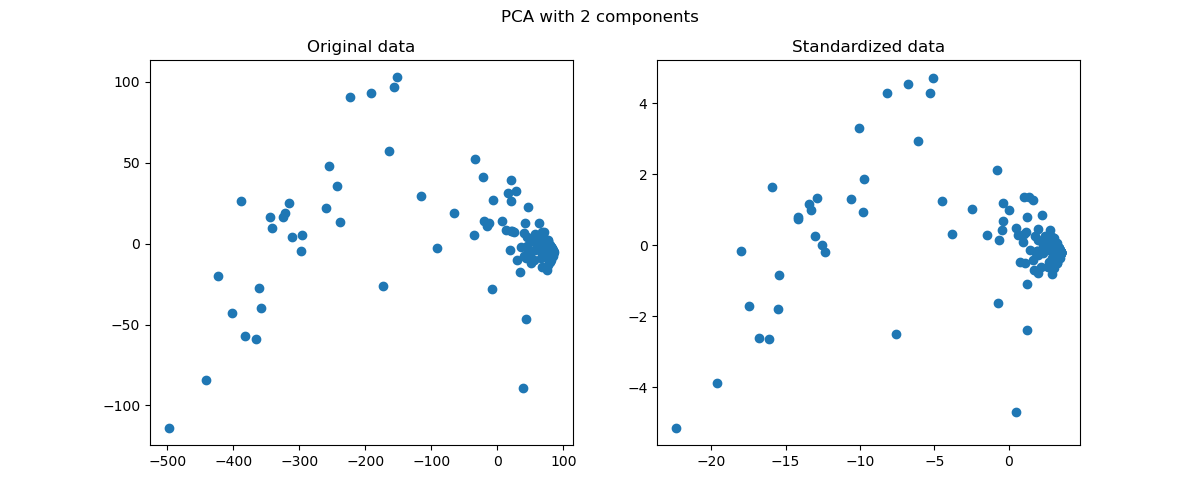
\includegraphics[width=1.0\linewidth]{reports/assignment-4/imgs/pca.png}
    \caption{Task 1 visualization (a)}
    \label{fig:pca}
\end{figure}

\begin{figure}[h]
    \centering
    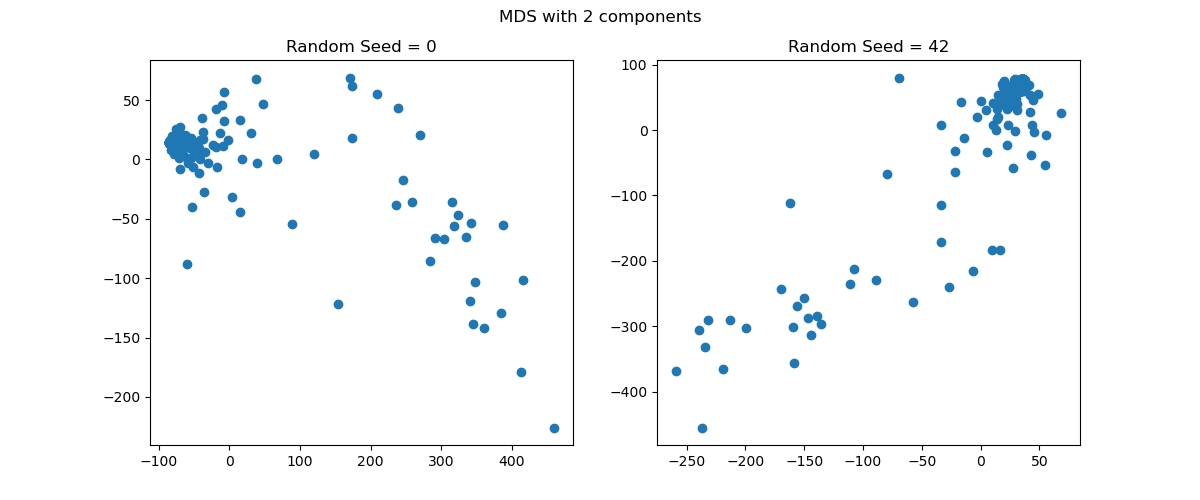
\includegraphics[width=1.0\linewidth]{reports/assignment-4/imgs/mds.png}
    \caption{Task 1 visualization (b)}
    \label{fig:mds}
\end{figure}

\begin{figure}[h]
    \centering
    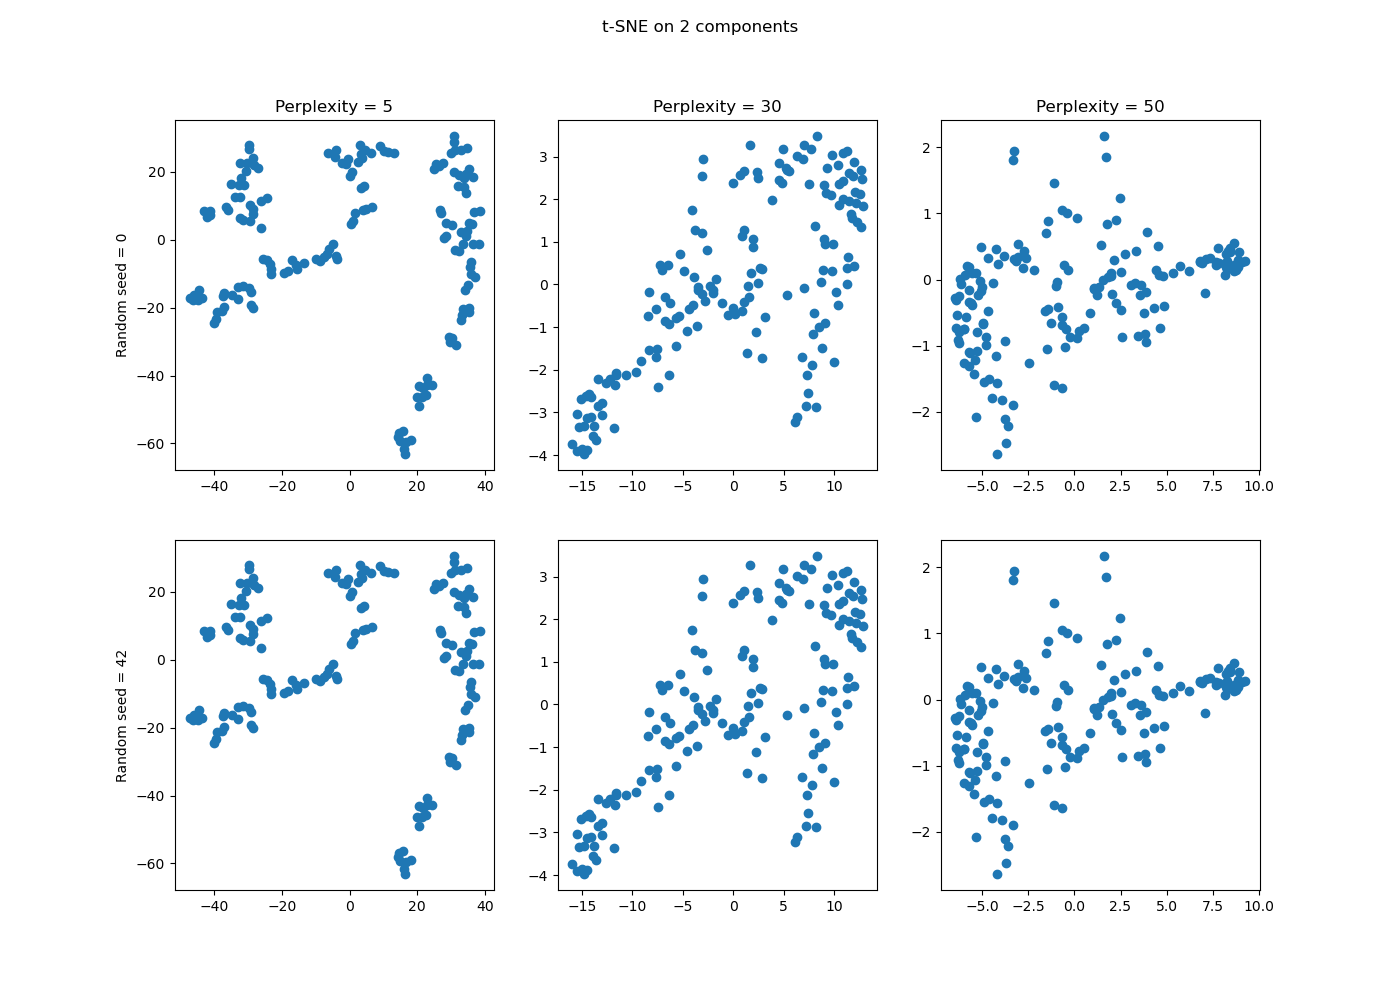
\includegraphics[width=1.0\linewidth]{reports/assignment-4/imgs/tsne.png}
    \caption{Task 1 visualization (c)}
    \label{fig:tsne}
\end{figure}

\section{Relational Data}

\begin{table}[h]
    \centering
    \renewcommand{\arraystretch}{1}
    \scalebox{0.7}{\begin{tabular}{c|ccccccccccccccccc}
        & 1 & 2 & 3 & 4 & 5 & 6 & 7 & 8 & 9 & 10 & 11 & 12 & 13 & 14 & 15 & 16 & 17 \\ \hline
      1  & 0 & 1 & 1 & 1 & 0 & 1 & 0 & 0 & 0 & 1 & 0 & 0 & 0 & 0 & 0 & 0 & 0 \\
      2  &   & 0 & 1 & 0 & 0 & 1 & 0 & 0 & 0 & 1 & 0 & 0 & 0 & 0 & 0 & 0 & 0 \\
      3  &   &   & 0 & 1 & 0 & 1 & 0 & 0 & 0 & 0 & 0 & 0 & 0 & 0 & 0 & 0 & 1 \\
      4  &   &   &   & 0 & 1 & 0 & 0 & 1 & 1 & 0 & 0 & 0 & 0 & 0 & 0 & 0 & 0 \\
      5  &   &   &   &   & 0 & 0 & 0 & 1 & 0 & 1 & 0 & 0 & 0 & 0 & 0 & 0 & 1 \\
      6  &   &   &   &   &   & 0 & 0 & 0 & 0 & 1 & 0 & 0 & 0 & 0 & 0 & 0 & 0 \\
      7  &   &   &   &   &   &   & 0 & 0 & 0 & 0 & 1 & 1 & 1 & 1 & 1 & 0 & 0 \\
      8  &   &   &   &   &   &   &   & 0 & 1 & 0 & 0 & 1 & 0 & 0 & 0 & 0 & 0 \\
      9  &   &   &   &   &   &   &   &   & 0 & 0 & 1 & 0 & 0 & 0 & 0 & 0 & 0 \\
     10  &   &   &   &   &   &   &   &   &   & 0 & 0 & 0 & 0 & 0 & 0 & 0 & 1 \\
     11  &   &   &   &   &   &   &   &   &   &   & 0 & 0 & 0 & 0 & 1 & 0 & 0 \\
     12  &   &   &   &   &   &   &   &   &   &   &   & 0 & 1 & 1 & 1 & 0 & 0 \\
     13  &   &   &   &   &   &   &   &   &   &   &   &   & 0 & 1 & 1 & 0 & 1 \\
     14  &   &   &   &   &   &   &   &   &   &   &   &   &   & 0 & 1 & 0 & 0 \\
     15  &   &   &   &   &   &   &   &   &   &   &   &   &   &   & 0 & 0 & 0 \\
     16  &   &   &   &   &   &   &   &   &   &   &   &   &   &   &   & 0 & 1 \\
     17  &   &   &   &   &   &   &   &   &   &   &   &   &   &   &   &   & 0 \\
    \end{tabular}
    }
    \caption{Adjacency matrix of SDGs}
    \label{adj}
\end{table}

\begin{figure}[h]
    \centering
    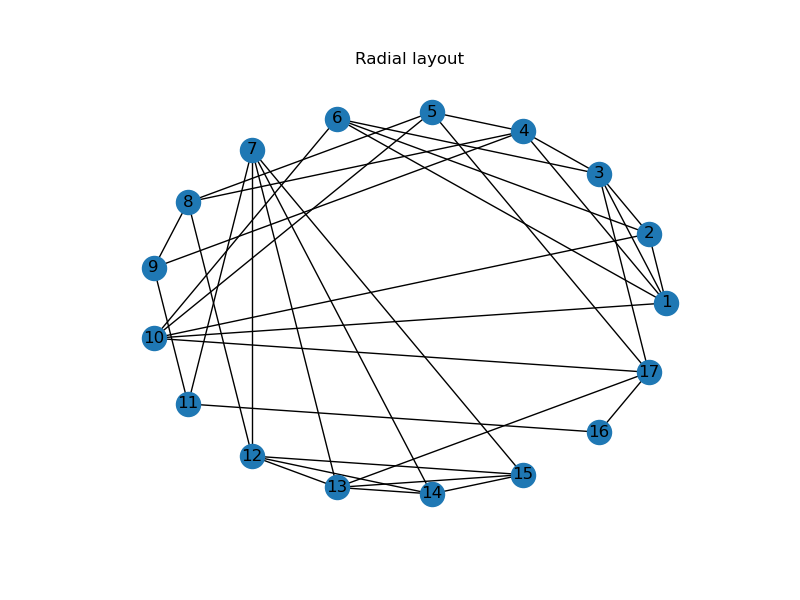
\includegraphics[width=1.0\linewidth]{reports/assignment-4/imgs/radial.png}
    \caption{Task 2 visualization (a)}
    \label{fig:rad}
\end{figure}

\begin{figure}[h]
    \centering
    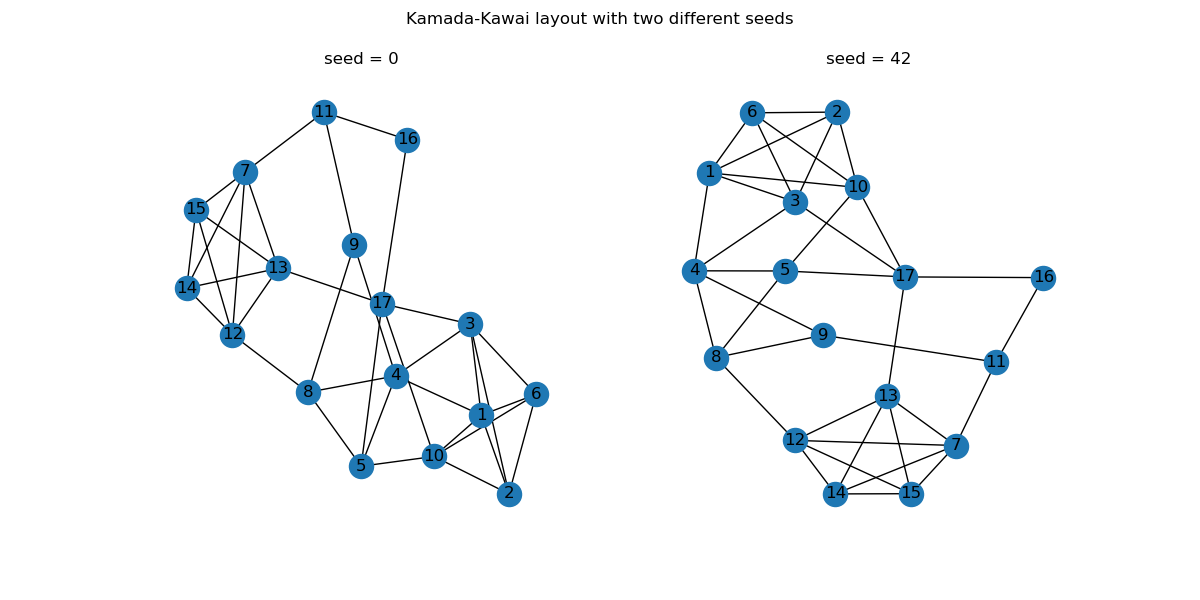
\includegraphics[width=1.0\linewidth]{reports/assignment-4/imgs/kk.png}
    \caption{Task 2 visualization (b)}
    \label{fig:kk}
\end{figure}

\begin{figure}[h]
    \centering
    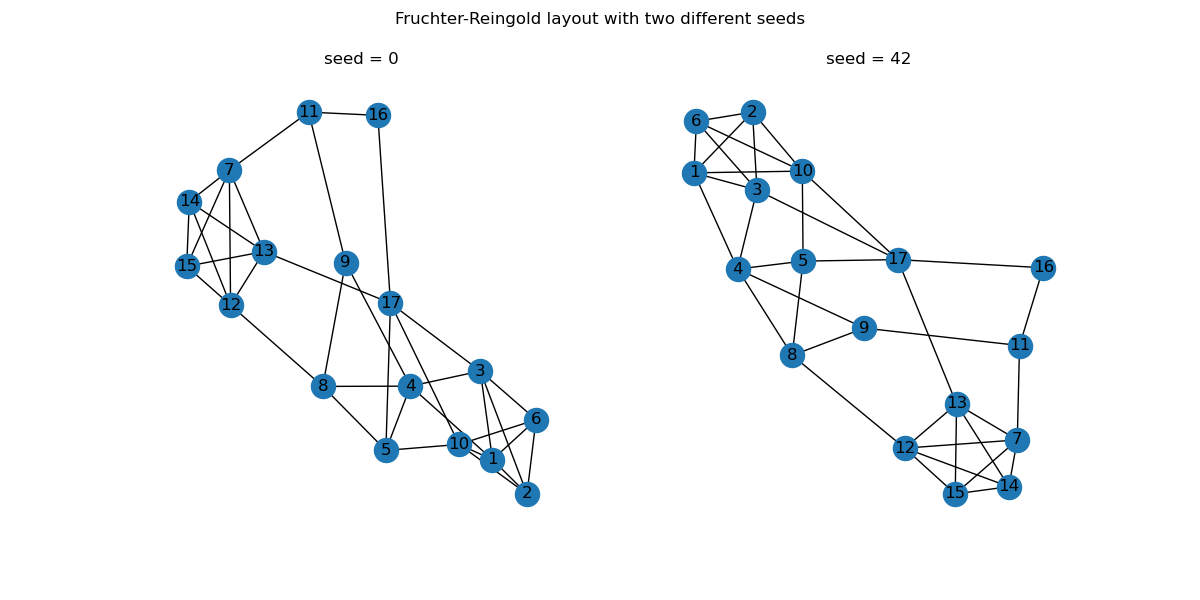
\includegraphics[width=1.0\linewidth]{reports/assignment-4/imgs/fr.png}
    \caption{Task 2 visualization (c)}
    \label{fig:fr}
\end{figure}

\newpage

\bibliography{reports/assignment-4/refs}

\end{document}